\documentclass{beamer}
\usepackage{beamerthemeAmsterdam}
\usepackage{amsmath}
\usepackage{graphicx}

\title{Wavelets 'n shit}
\subtitle{}
\author{Jan Westerdiep \and Okke van Garderen}
\date{\today}
\institute{Universiteit van Amsterdam}

\renewcommand{\figurename}{}

\begin{document}

\frame{\titlepage}

\frame{
\frametitle{Fourier Transformatie}
\begin{columns}  \begin{column}{0.5\linewidth}\begin{itemize}
    \item
    \item
    \item
\end{itemize}  \end{column}\begin{column}{0.5\linewidth}
    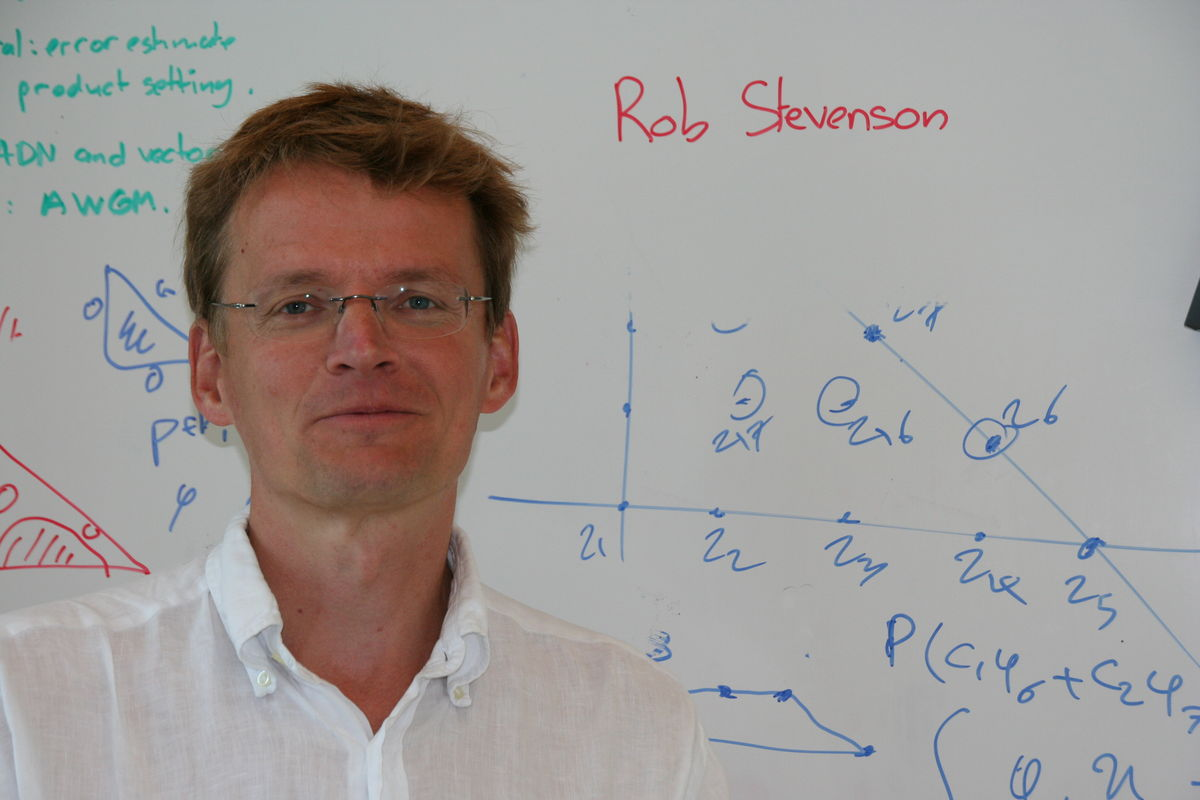
\includegraphics[width=\linewidth]{robbierobrob.jpg}
\end{column}\end{columns}
}

\frame{
\frametitle{}
\begin{columns}  \begin{column}{0.5\linewidth}\begin{itemize}
    \item
    \item
    \item
\end{itemize}  \end{column}\begin{column}{0.5\linewidth}
    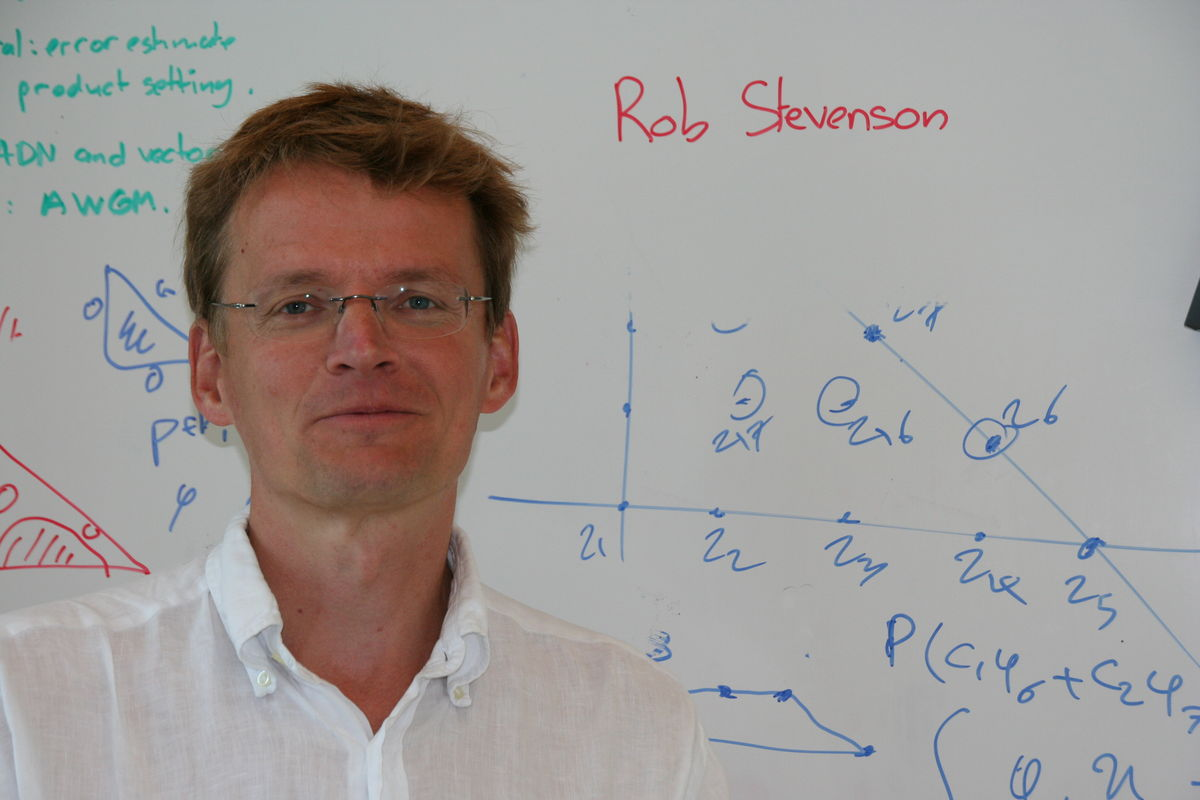
\includegraphics[width=\linewidth]{robbierobrob.jpg}
\end{column}\end{columns}
}

\frame{
\frametitle{Begeleider: Rob Stevensson}
\begin{columns}
  \begin{column}{0.5\linewidth}
    \begin{itemize}
    \item was numerieke analyse docent
    \item alles wat ie doet heeft met wavelets te maken
    \item ALLES wat ie doet heeft met wavelets te maken
    \end{itemize}
  \end{column}
  \begin{column}{0.5\linewidth}
    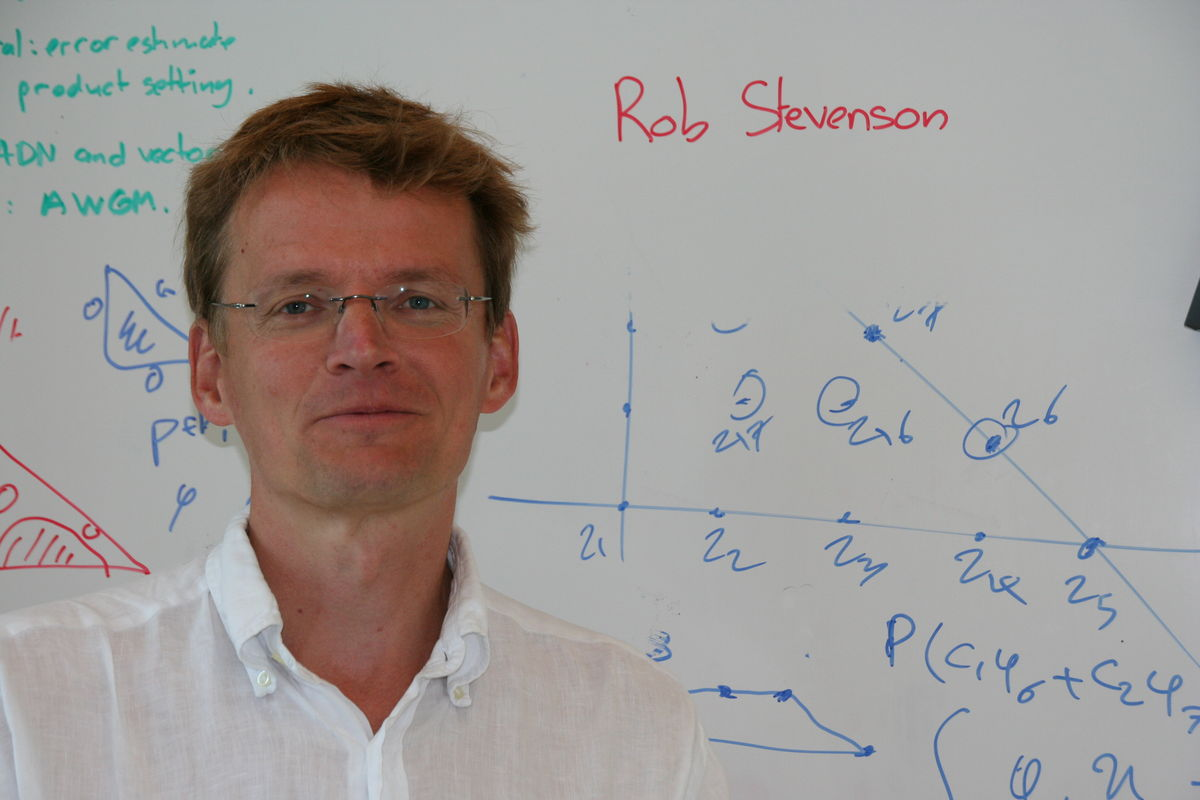
\includegraphics[width=\linewidth]{robbierobrob.jpg}
  \end{column}
\end{columns}
}

\frame{
\frametitle{Jan is een neger}

\includegraphics[height=\linewidth]{JPEGthestrongest.jpg}
}

\end{document}
